% arara: pdflatex
% !arara: indent: {overwrite: yes, trace: yes}
\documentclass[10pt]{article}
\usepackage[margin=.5cm,left=0cm,foot=0cm,bottom=0cm]{geometry}
\usepackage{ifthen}
\usepackage{tikz}
\usepackage{kpfonts}
\usetikzlibrary{matrix}
\usetikzlibrary{shapes}
\usetikzlibrary{decorations}
\usetikzlibrary{decorations.markings}

\makeatletter
\newcommand{\cmh}[1]{%
	\@ifundefined{c@totalpoints}%
	{%
		\newcounter{totalpoints}
		\setcounter{totalpoints}{#1}
		\typeout{Defining a new counter: totalpoints}
	}%
	{%
		\ifnum\value{totalpoints}=#1
			\typeout{Total points match auxilary file (#1)}
		\else
			\typeout{Warning: total points updated from \the\value{totalpoints} to #1-- recompile to fix}
		\fi
		\setcounter{totalpoints}{#1}
	}%
}
\AtEndDocument{%
	\immediate\write\@auxout{%
		\string\cmh\string{\the\value{totalpoints@tmp}\string}%
	}
}

\newcounter{totalpoints@tmp}
\newcommand{\points}[1]{%
	\ifthenelse{\equal{#1}{bronze}}{10\addtocounter{totalpoints@tmp}{10}}{}%
	\ifthenelse{\equal{#1}{silver}}{20\addtocounter{totalpoints@tmp}{20}}{}%
	\ifthenelse{\equal{#1}{gold}}{30\addtocounter{totalpoints@tmp}{30}}{}%
	\ifthenelse{\equal{#1}{level}}{+}{}%
}

\tikzset{
	empty/.style={
		draw=gray,
		star,
		anchor=center,
		scale=2,
	},
	badge/.style={
		scale=1.2,
		text=white,
		fill=black!70,
		rounded corners=1ex,
		text width=4cm,
		minimum width=3cm,
		minimum height=0.9cm,
		align=right,
		font=\bfseries,
		decoration={
			markings,% switch on markings
			mark=% actually add a mark
			at position 0cm
			with
			{
				\coordinate (cmh) at (127pt,18pt);
				\node[
					draw=white,
					double,
					#1,
					align=center,
					text=black,
				scale=.15,] at (cmh) {\resizebox{2.5cm}{!}{\points{#1}}};
			}
		},
		postaction=decorate,
	},
	badge/.default=bronze,
	description/.style={
		font=\itshape,
	},
	bronze/.style={circle,fill=bronze},
	silver/.style={rounded corners=0ex,fill=silver, minimum height=2.6cm},
	gold/.style={isosceles triangle,fill=gold},
	level/.style={circle,fill=cyan},
	mymatrix/.style={
		matrix of nodes,
		nodes in empty cells,
		column sep=.1cm,
		execute at empty cell={\node[empty]{};},
		every even row/.style={nodes={description}},
	}
}


% define colours for the badges
\colorlet{bronze}{brown!20!orange}
\colorlet{silver}{gray!30!white}
\colorlet{gold}{yellow!90!white}

% page style, title
\pagestyle{empty}
\title{Achievements}
\author{Math 65}
\date{}



\begin{document}

\makeatletter
\@ifundefined{c@totalpoints}%
{%
	\def\mybase{\relax}
	\def\mymultiplier{\relax}
}%
{%
	% formula for the levels
	%       f(x) = a * b^x
	%
	\pgfmathsetmacro{\levelOnePoints}{30}
	\pgfmathparse{(\the\value{totalpoints}/\levelOnePoints)^(1/9)}
	% b
	\pgfmathsetmacro{\mybase}{\pgfmathresult}
	% a
	\pgfmathsetmacro{\mymultiplier}{\levelOnePoints/(\mybase)}
}

% compute the points at each level
\newcommand{\levelpts}[1]{%     #1: level
	\@ifundefined{c@totalpoints}%
	{%
		??%
	}%
	{%
		\pgfmathparse{\mymultiplier*(\mybase)^#1}%
		\pgfmathprintnumber{\pgfmathresult}%
	}%
}

% counter for the levels
\newcounter{level}
\newcommand{\steplevel}{\stepcounter{level}\thelevel}

\maketitle

\pgfkeys{/pgf/number format/.cd,fixed,precision=0}

\begin{minipage}{.33\textwidth}
	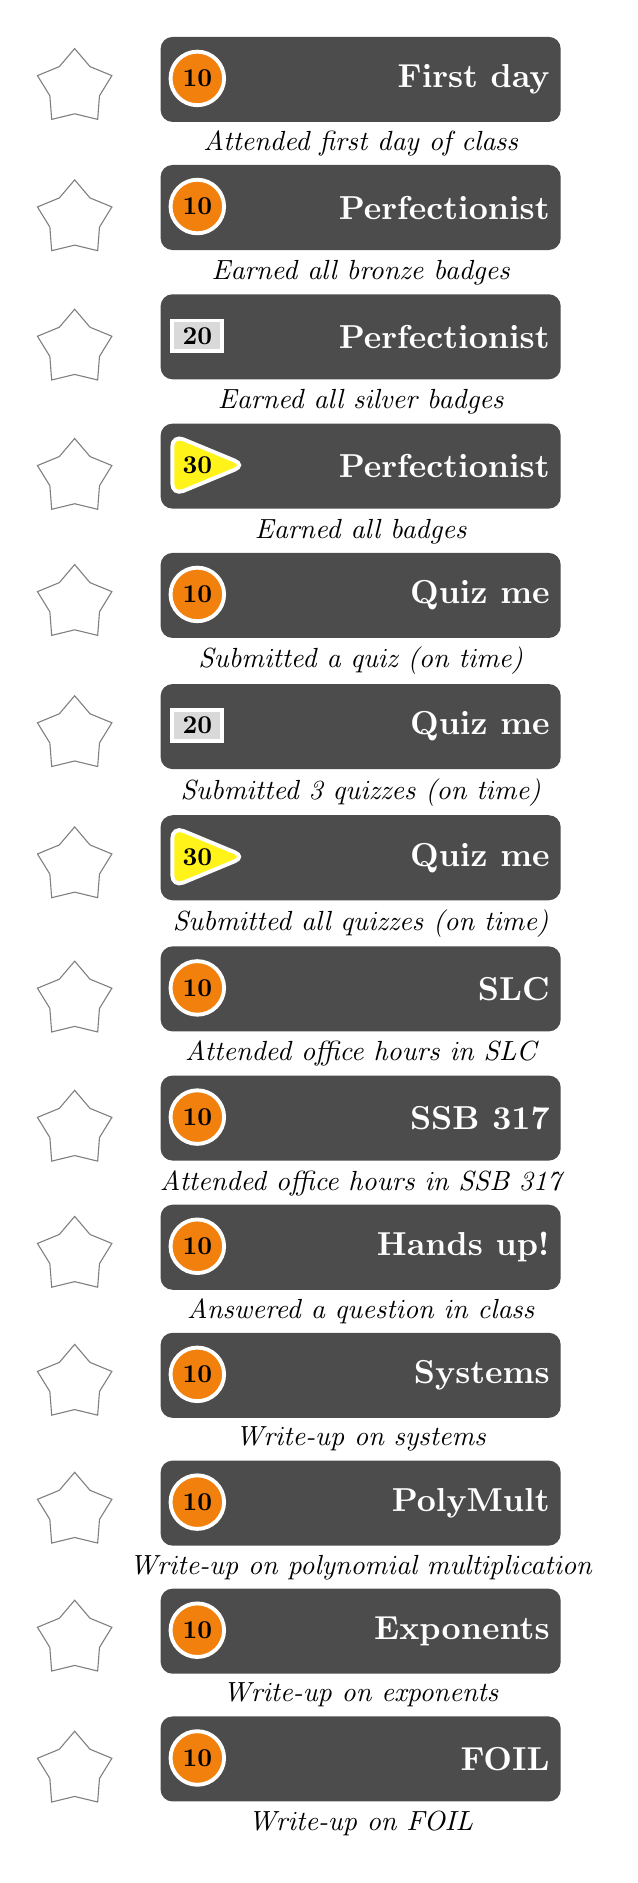
\begin{tikzpicture}
		\matrix[mymatrix]{
			%* \begin{tabular}
			   & |[badge]|First day                    \\
			{} & Attended first day of class           \\
			   & |[badge]|Perfectionist                \\
			{} & Earned all bronze badges              \\
			   & |[badge=silver]|Perfectionist         \\
			{} & Earned all silver badges              \\
			   & |[badge=gold]|Perfectionist           \\
			{} & Earned all badges                     \\
			   & |[badge]| Quiz me                     \\
			{} & Submitted a quiz (on time)            \\
			   & |[badge=silver]| Quiz me              \\
			{} & Submitted 3 quizzes (on time)         \\
			   & |[badge=gold]| Quiz me                \\
			{} & Submitted all quizzes (on time)       \\
			   & |[badge]| SLC                         \\
			{} & Attended office hours in SLC          \\
			   & |[badge]| SSB 317                     \\
			{} & Attended office hours in SSB 317      \\
			   & |[badge]| Hands up!                   \\
			{} & Answered a question in class          \\
			   & |[badge]|Systems                      \\
			{} & Write-up on systems                   \\
			   & |[badge]|PolyMult                     \\
			{} & Write-up on polynomial multiplication \\
			   & |[badge]|Exponents                    \\
			{} & Write-up on exponents                 \\
			   & |[badge]|FOIL                         \\
			{} & Write-up on FOIL                      \\
			%* \end{tabular}
		};
	\end{tikzpicture}
\end{minipage}%
\begin{minipage}{.33\textwidth}
	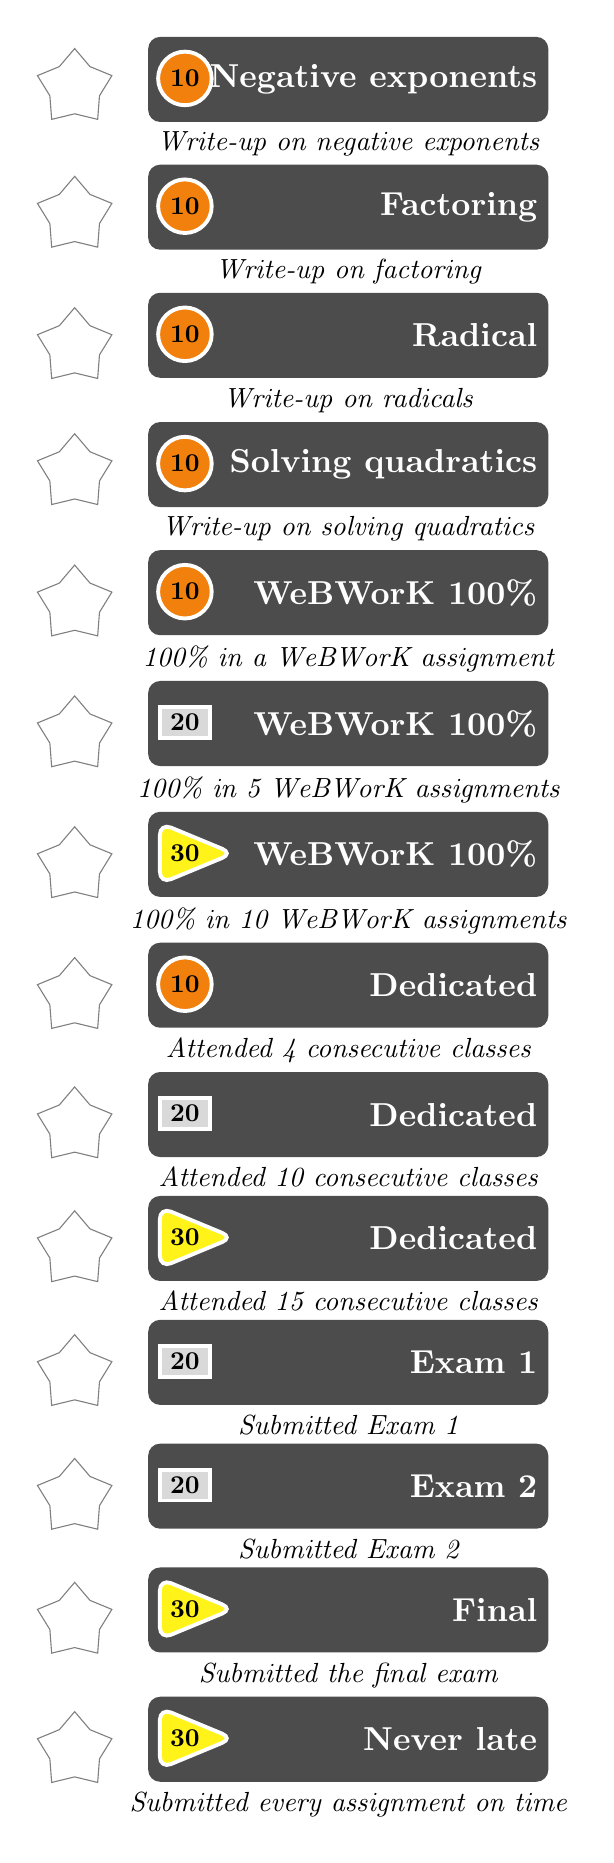
\begin{tikzpicture}
		\matrix[mymatrix]{
			%* \begin{tabular}
			   & |[badge]|Negative exponents        \\
			{} & Write-up on negative exponents     \\
			   & |[badge]|Factoring                 \\
			{} & Write-up on factoring              \\
			   & |[badge]|Radical                   \\
			{} & Write-up on radicals               \\
			   & |[badge]|Solving quadratics        \\
			{} & Write-up on solving quadratics     \\
			   & |[badge]|WeBWorK 100\%             \\
			{} & 100\% in a WeBWorK assignment      \\
			   & |[badge=silver]|WeBWorK 100\%      \\
			{} & 100\% in 5 WeBWorK assignments     \\
			   & |[badge=gold]|WeBWorK 100\%        \\
			{} & 100\% in 10 WeBWorK assignments    \\
			   & |[badge]| Dedicated                \\
			{} & Attended 4 consecutive classes     \\
			   & |[badge=silver]| Dedicated         \\
			{} & Attended 10 consecutive classes    \\
			   & |[badge=gold]| Dedicated           \\
			{} & Attended 15 consecutive classes    \\
			   & |[badge=silver]| Exam 1            \\
			{} & Submitted Exam 1                   \\
			   & |[badge=silver]| Exam 2            \\
			{} & Submitted Exam 2                   \\
			   & |[badge=gold]|Final                \\
			{} & Submitted the final exam           \\
			   & |[badge=gold]|Never late           \\
			{} & Submitted every assignment on time \\
			%* \end{tabular}
		};
	\end{tikzpicture}
\end{minipage}%
\begin{minipage}{.33\textwidth}
	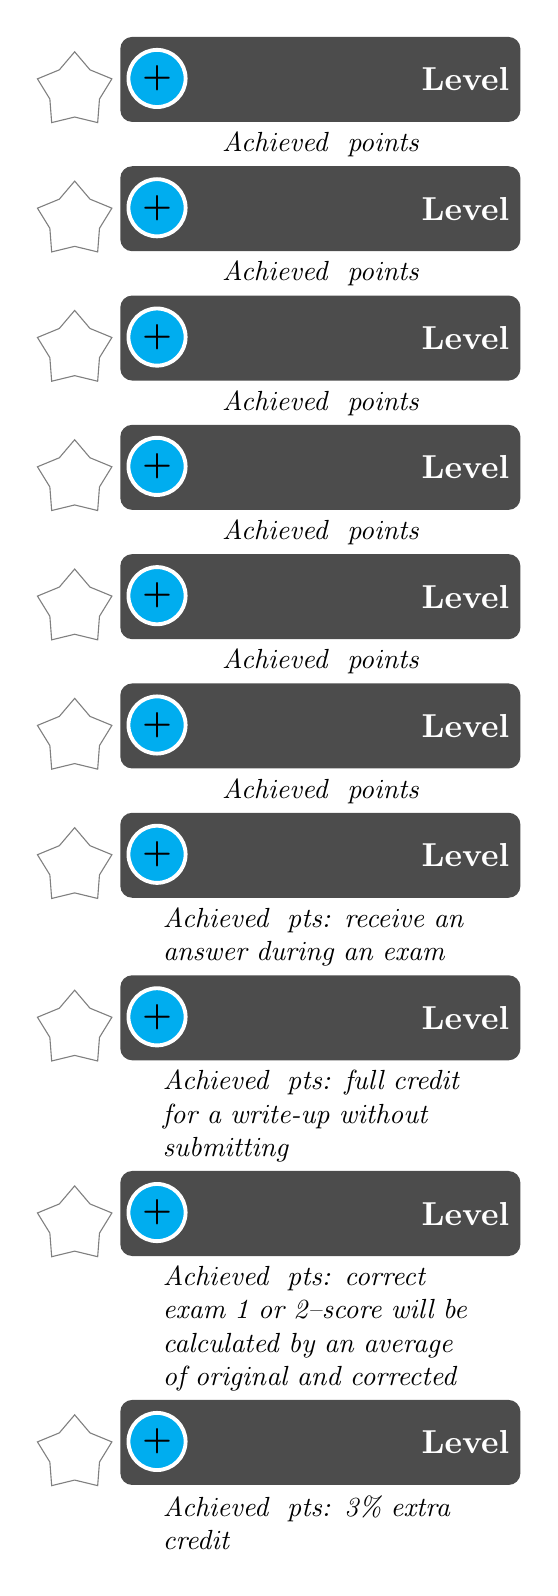
\begin{tikzpicture}
		\matrix[mymatrix]{
			%* \begin{tabular}
			   & |[badge=level]|Level \steplevel                                                                                                            \\
			{} & Achieved \levelpts{\thelevel} points                                                                                                       \\
			   & |[badge=level]|Level \steplevel                                                                                                            \\
			{} & Achieved \levelpts{\thelevel} points                                                                                                       \\
			   & |[badge=level]|Level \steplevel                                                                                                            \\
			{} & Achieved \levelpts{\thelevel} points                                                                                                       \\
			   & |[badge=level]|Level \steplevel                                                                                                            \\
			{} & Achieved \levelpts{\thelevel} points                                                                                                       \\
			   & |[badge=level]|Level \steplevel                                                                                                            \\
			{} & Achieved \levelpts{\thelevel} points                                                                                                       \\
			   & |[badge=level]|Level \steplevel                                                                                                            \\
			{} & Achieved \levelpts{\thelevel} points                                                                                                       \\
			   & |[badge=level]|Level \steplevel                                                                                                            \\
			{} & |[text width=4cm]|Achieved \levelpts{\thelevel} pts: receive an answer during an exam                                                      \\
			   & |[badge=level]|Level \steplevel                                                                                                            \\
			{} & |[text width=4cm]|Achieved \levelpts{\thelevel} pts: full credit for a write-up without submitting                                         \\
			   & |[badge=level]|Level \steplevel                                                                                                            \\
			{} & |[text width=4cm]|Achieved \levelpts{\thelevel} pts: correct exam 1 or 2--score will be calculated by an average of original and corrected \\
			   & |[badge=level]|Level \steplevel                                                                                                            \\
			{} & |[text width=4cm]|Achieved \levelpts{\thelevel} pts: 3\% extra credit                                                                      \\
			%* \end{tabular}
		};
	\end{tikzpicture}

	Total points available: \thetotalpoints@tmp
\end{minipage}%


\end{document}
